\documentclass
[
	paper = a4,
    pagesize,
	12 pt,
	oneside,                       % Chose ›oneside‹ for digital version, ›twoside‹ for printed version.
    open = right,
	DIV = calc,
	BCOR = 0 mm,                   % Binding correction. Only necessary for printed version. Depends on actual binding.
	bibtotoc
]
{scrbook}

% Do not change the following commands.
\newcommand*{\printTitle}{}
\newcommand*{\printAuthor}{}
\newcommand*{\printDateOfBirth}{}
\newcommand*{\printPlaceOfBirth}{}
\newcommand*{\printSubject}{}
\newcommand*{\myTitle}[1]{\renewcommand*{\printTitle}{#1}}
\newcommand*{\myName}[1]{\renewcommand*{\printAuthor}{#1}}
\newcommand*{\myDateOfBirth}[1]{\renewcommand*{\printDateOfBirth}{#1}}
\newcommand*{\myPlaceOfBirth}[1]{\renewcommand*{\printPlaceOfBirth}{#1}}
\newcommand*{\mySubject}[1]{\renewcommand*{\printSubject}{#1}}

\myTitle{High-Level visualization of graph algorrithms}  % Change!
\myName{Julius Milian Severin}  % Change!
\myDateOfBirth{March~12, 1995}  % Change!
\myPlaceOfBirth{Berlin, Germany}  % Change!
\mySubject{{Graph Algorithms}{Visualization}}  % Change!

\usepackage[utf8]{inputenc}
\usepackage[T1]{fontenc}
\usepackage[english]{babel}

\usepackage{graphicx}

\graphicspath{{Images/}}

\usepackage{pgf}

\usepackage							% Microtypography tuning.
[
	protrusion = true,
	expansion = false,
	tracking = true,
	kerning = true,
	spacing = false,
	babel = true
]
{microtype}							% http://ctan.mirrorcatalogs.com/macros/latex/contrib/microtype/microtype.pdf

\SetTracking[unit = space]{font = */*/*/sc/*}{25}   % Adjust kerning for small caps.

\SetExtraKerning[unit = space]		% Adjusted kerning for certain characters.
{
	font = */*/*/*/*
}
{
	: = {100, },
	; = {100, },
	? = {150, 150},
	! = {150, 150},
	: = {250, },
	; = {150, },
	? = {250, 250},
	! = {250, 250},
	» = { , -200},
	« = {-200, },
	› = { , -200},
	‹ = {-200, },
	– = {200, 250},
	— = {200, 250},
	@ = {200, 200}
}

\usepackage{booktabs}
\usepackage{breakurl}
\usepackage{emptypage}

\usepackage[bottom]{footmisc}
\usepackage{remreset}

\makeatletter
    \@removefromreset{footnote}{chapter}
\makeatother

\renewcommand*{\footnoterule}{\rule{0 pt}{0 pt}}
\deffootnote[1.2 em]{1.2 em}{0 em}{\makebox[1.4 em][l]{\textbf{\thefootnotemark}}}

\usepackage{xparse}

\DeclareDocumentCommand{\myfootnote}{o o o m}
{%
    \IfNoValueTF{#1}%
    {%
        \footnote{#4}%
    }%
    {%
        \IfNoValueTF{#2}%
        {%
            \kern #1 em\footnote{#4}%
        }%
        {%
            \IfNoValueTF{#3}%
            {%
                \kern #1 em\footnote{#4}\kern #2 em%
            }%
            {%
                \kern #1 em\footnote[#3]{#4}\kern #2 em%
            }%
        }%
    }%
}

\usepackage{titlesec}

\titleformat{\chapter}
    {\normalfont\rmfamily\huge\bfseries}
    {\thechapter}{1 em}{}

\titleformat{\section}
    {\normalfont\rmfamily\Large\bfseries}
    {\thesection}{1 em}{}

\titleformat{\subsection}
    {\normalfont\rmfamily\large\bfseries}
    {\thesubsection}{1 em}{}

\titleformat{\subsubsection}
    {\normalfont\rmfamily\normalsize\bfseries}
    {\subsubsectionname}{1 em}{}


\pagestyle{headings}

\usepackage{amsmath}
\usepackage{amssymb}
\usepackage{amsfonts}
%\usepackage{upgreek}               % Use if you want to use upright lowercase and italic upercase greek letters.
%\usepackage{dsfont}                % Use if you want to use special symbols.

%\usepackage[printonlyused]{acronym} % Use if you want to have acronyms. http://mirror.hmc.edu/ctan/macros/latex/contrib/acronym/acronym.pdf

%\usepackage{pifont}				% Special symbols.
%\usepackage{fourier-orns}			% More special symbols.
\usepackage{lettrine}

\usepackage{enumitem}
\usepackage
[
	format = plain,
	textfont = {sf, footnotesize},
	labelfont = {sf, bf}
]
{caption}[2008/08/24]
\usepackage{subcaption}				% For using sub-figures.

\usepackage
[
    algo2e,
    ruled,
    vlined,
    linesnumbered,
    algochapter
]
{algorithm2e}

\SetAlCapFnt{\sffamily\footnotesize}
\SetAlCapNameFnt{\sffamily\footnotesize}

\usepackage[numbers]{natbib}

\makeatletter
    \def\NAT@spacechar{~}% NEW
\makeatother

\definecolor{darkblue}{rgb}{0, 0, 0.5}

\usepackage
[
	bookmarks = true,
	bookmarksopen = false,
	bookmarksnumbered = true,
	pdfstartpage = 1,
	pdftitle = {{\printTitle}},
	pdfauthor = {{\printAuthor}},
	pdfsubject = {{\printSubject}},
	backref = page,
	breaklinks = true,
	colorlinks = true,
	linkcolor = darkblue,
	anchorcolor = darkblue,
	citecolor = darkblue,
	filecolor = darkblue,
	menucolor = darkblue,
	pagecolor = darkblue,
	urlcolor = darkblue
]

\usepackage{hyperref}


\renewcommand*{\backref}[1]{}
\renewcommand*{\backrefalt}[4]
{
    \ifcase #1
        Not cited.
    \or
        \footnotesize (Cited on page #2.)
    \else
        \footnotesize (Cited on pages #2.)
    \fi
}

\usepackage{cleveref}

\begin{document}




\begin{document}


\frontmatter
% Title Page
\thispagestyle{empty}
\begin{center}
    {\Huge \textbf{\printTitle}}\\[7 ex]
    {\Large\textsc{Bachelor Thesis}}\\[4 ex]    
    {\large
        to attain the scientific degree\\[4 ex]
        \textbf{Bachelor of Science}
    }
    \vfill
    \includegraphics[width = 8 cm]{HPI_logo.pdf}\\[8 ex]
    \begin{tabular}{l}
        handed in by \textbf{\printAuthor}\\[1.1 ex]
        born \printDateOfBirth, in \printPlaceOfBirth\\[3 ex]
        \textbf{Advisor:} Prof.~Dr.~Tobias Friedrich\\[9 ex]
    \end{tabular}
    
    Potsdam, \today
\end{center}

% Abstract
\chapter*{}
\addcontentsline{toc}{chapter}{Abstract}
\thispagestyle{empty}

\begin{center}
    \large \textbf{Abstract}
\end{center}

Developing an algorithm is an iterative process.
Therefore an understanding of the different approches is important.
Furthermore, as the algorithm becomes more complex, it may come to different results than expected, when running on real data.

This thesis deals with those issues on the example of shortest path algorithm on tiled map data.
Therefore, multiple ways of visualizing a shortest path algorithm with respect of this specific class of algorithms are introduced.
Using those methods we were able to archieve a better understanding of the algorithms and built a powerful basis for discussions.
In addition we enabled the researchers to find the missbehaviour more easily.

\chapter*{}
\addcontentsline{toc}{chapter}{Zusammenfassung}
\thispagestyle{empty}

\begin{center}
    \large \textbf{Zusammenfassung}
\end{center}

Das Entwickeln eines Algorithmusses ist ein iterativer Prozess.
Daher ist es wichitg, dass alle Beteiligten, die verschiedenen Ansätze verstehen.
Ausserdem kann es mit wachsender Komplexität des Algoithmus dazu kommen, dass sich der Algorithmus auf echten Daten anders verhalten als gedacht.
Das finden der Ursache kann ein äußerst komplexes Verfahren sein.

In der folgenden Arbeit erklären wir, wie wir die Entwicklung eines Algorithmus zum finden kürzester Wege durch eine Visualisierung untersützt haben.
Dabei gehen wir auf die Probleme ein, die wir wärend der Entwicklung der Visualisierung lösen mussten.


% Table of Contents
\renewcommand*{\listfigurename}{\normalfont\rmfamily\Large\bfseries List of Figures}
\renewcommand*{\listtablename}{\normalfont\rmfamily\Large\bfseries List of Tables}
\pdfbookmark{\contentsname}{toc}
\microtypesetup{protrusion = false}
    \tableofcontents
    \begingroup
    \let\clearpage\relax
    \listoffigures                  % Comment out if necessary.
    \listoftables                   % Comment out if necessary.
    \endgroup
\microtypesetup{protrusion = true}


\mainmatter
\chapter{Introduction} \label{introduction}
Graphs are a common structure in computer science.
Therefore developing more efficient graph algorithms plays a big role in algorithm engineering.
During the process of development knowing how the algorithm behaves is really important.
Firstly developing an algorithm is an iterative process it is fundamental to communicate about the different approaches and therefore create an understanding of them in the whole team.
Furthermore, the developed algorithms can become quite complex and therefore the idea of how the algorithms should behave and the way they actually behave on real graph data can diverge quite a lot.
\par
As the eyes are a fast way to access information a good way to achieve this understanding is to visualize the progress of the algorithm.
Though there are many tools for visualizing graphs, there is still a lack of algorithm visualization tools.
Therefore writing an own visualization that fits one's needs might be necessary.
In the following, we will describe the process of developing a sensemaking visualization the example of a shortest path algorithm. The algorithm was developed on a geographical tiled road network with the special requirement to reduce the amount of tile-accesses during the algorithm.

\chapter{Prelimanaries} \label{questions}

This chapter starts by giving all important information about the graph and the specification of the algorithm itself followed by a selection of questions that came up during the process of developing the visualization.


\section{Problem Specification} \label{specification}
% \begin{itemize}
%     \item Knoten
%     \begin{itemize}
%         \item mit Koordinaten versehen
%     \end{itemize}
%     \item Kanten
%     \begin{itemize}
%         \item gerichtet
%         \item mit Geschwindigkeit + Länge
%     \end{itemize}
% \end{itemize}

Before we start building our visualization, we are going to take a look at the graph the algorithms will be running on.
As a geographical graph is given, every node has some coordinates according to its position on the earth.
The edges are directed and weighted, whereby the weight is given by length and speed.
In \ref{introduction} we already mentioned tiles.
Those tiles have been introduced by the Navigation Data Standart (NDS). It divides the graph according to a geographical grid.
Therefore every tile is bounded by a coordinate on every site.
As the tiles are encrypted and compressed the costs for loading them are the main cost factor during the algorithm.



\section{Displaying the Graph} \label{graph}

% \begin{itemize}
%     \item Wie ordnet man Knoten an?
%     \begin{itemize}
%         \item Koordinaten
%     \end{itemize}
%     \item Wie repräsentiert man Knoten?
%     \begin{itemize}
%         \item Kreise
%         \item keine explizite Darstellung -> start und End von Kante
%     \end{itemize}
%     \item Wie repräsentiert man Kanten?
%     \begin{itemize}
%         \item Linie
%     \end{itemize}
% \end{itemize}

When trying to visualize a graph algorithm a good start is to think about a way to display the graph itself first.
Therefore it is necessary to find a way to arrange the nodes and think about a way to represent nodes and edges in general.



\section{Displaying the Algorithm}

Even though visualizing graphs on a high level is a common thing and impressive graphs is a even used for marketing reasons (e.g. Facebook), visualizing algorithms itself is mostly seen in doctrine on a small scale.

\subsection{Basics}

% \begin{itemize}
%     \item Welcher Bereich ist am Anfang im Bild?
%     \begin{itemize}
%         \item Zentrum
%         \begin{itemize}
%             \item Start
%             \item Mitte zwischen Start + Ziel
%             \item Mitte der Suchfront
%         \end{itemize}
%     \end{itemize}
%     \item Welche Features sind noch Sinnvoll/nötig? // vielleicht eher zum Fazit?
%     \begin{itemize}
%         \item Zoom + Bewegen
%         \item Schrittweise vor/zurück (je nach visualisiertem)
%     \end{itemize}
% \end{itemize}

Since the visualization of graph algorithms is not such common, there are multiple basic questions that need to be answered.
Which segment should be shown in the beginning? How to visualize the progressing algorithm?
And which basic features should be included for increasing the accessibility of the information displayed.
\todo{how to display start and end}
\todo{Maybe put this to Micellaneous}

\subsection{Displaying the Tiles}

% \begin{itemize}
%     \item  Wie werden Tiles repäsentiert?
%     \begin{itemize}
%         \item Durch alle enthaltenden Kanten
%         \item Durch Rechtecke
%     \end{itemize}
% \end{itemize}

The in \ref{specification} we already introduced the tiles that play a major role in the algorithms developed.
Therefore we need to find a way to make the tiles visible for the user.


\subsection{Visualizing the Cache}

% \begin{itemize}
%     \item Wie kann man den Cache Visualisieren?
%     \begin{itemize}
%         \item Einfärbung der aktuell geladenen Tiles
%     \end{itemize}
%     \item Wie kann man Mehrfachladungen repräsentieren?
%     \begin{itemize}
%         \item Farbe
%         \begin{itemize}
%             \item Weiß zu Rot
%             \item Grün zu Rot
%         \end{itemize}
%     \end{itemize}
% \end{itemize}

In the algorithms that should be developed the cache plays a role as well.
Tiles only need to be loaded when they are not in the cache yet.
So the relevant information is not how often a tile is accessed but how often a tile is accessed when it was not in the cache before.
Hence we need to find a way to display that information as well.


\section{Compare algorithms}

% \begin{itemize}
%     \item Wie kann man mehrere Algorithmen miteinander vergleichen?
%     \begin{itemize}
%         \item Nebeneinander laufen lassen
%         \item Entergebnis vergleichen
%         \item Differenz anzeigen
%     \end{itemize}
% \end{itemize}

After having answered all those questions introduced in the previous chapters we might also want to compare different algorithms. Is there maybe a way that includes more than just starting the visualization with two different algorithms and put them next to each other?



\section{Miscellaneous}

% \begin{itemize}
%     \item Welche Features sind noch sinnvoll?
%     \begin{itemize}
%         \item Bei Bedarf Graph einblenden
%         \begin{itemize}
%             \item Einfarbig
%             \item Farben als repräsentierung von Geschwindigkeiten
%         \end{itemize}
%     \end{itemize}
% \end{itemize}

In the end we will discuss some additional fancy features to give the visualization the last fancy touch.



\chapter{Buillding the Visualization}

In this chapter we will discuss the questions introduced in \ref{questions}.


\section{Displaying the Graph}

This section we will take a closer look at the problematics introduced in \ref{graph} starting by the problem of aranging the nodes.
As every node has given unique coordinates we will use those to arrange them on the screen.
Therefore there are already many projections that calculate the position on the screen for given coordinates.
The porbably most intuitive way of projecting coordinates is to just see the longitude and the latitude as coordinates on a two-dimensional graph.
This projection is called Equirectangular projection.
\par
An other common projection is the Mercator Porjection.
In Mercator projection the longitudes are all equally spaced but the latitudes move away from each other the bigger the distance to the equator becomes.

\todo{center the first image}

\begin{figure}[h!]
	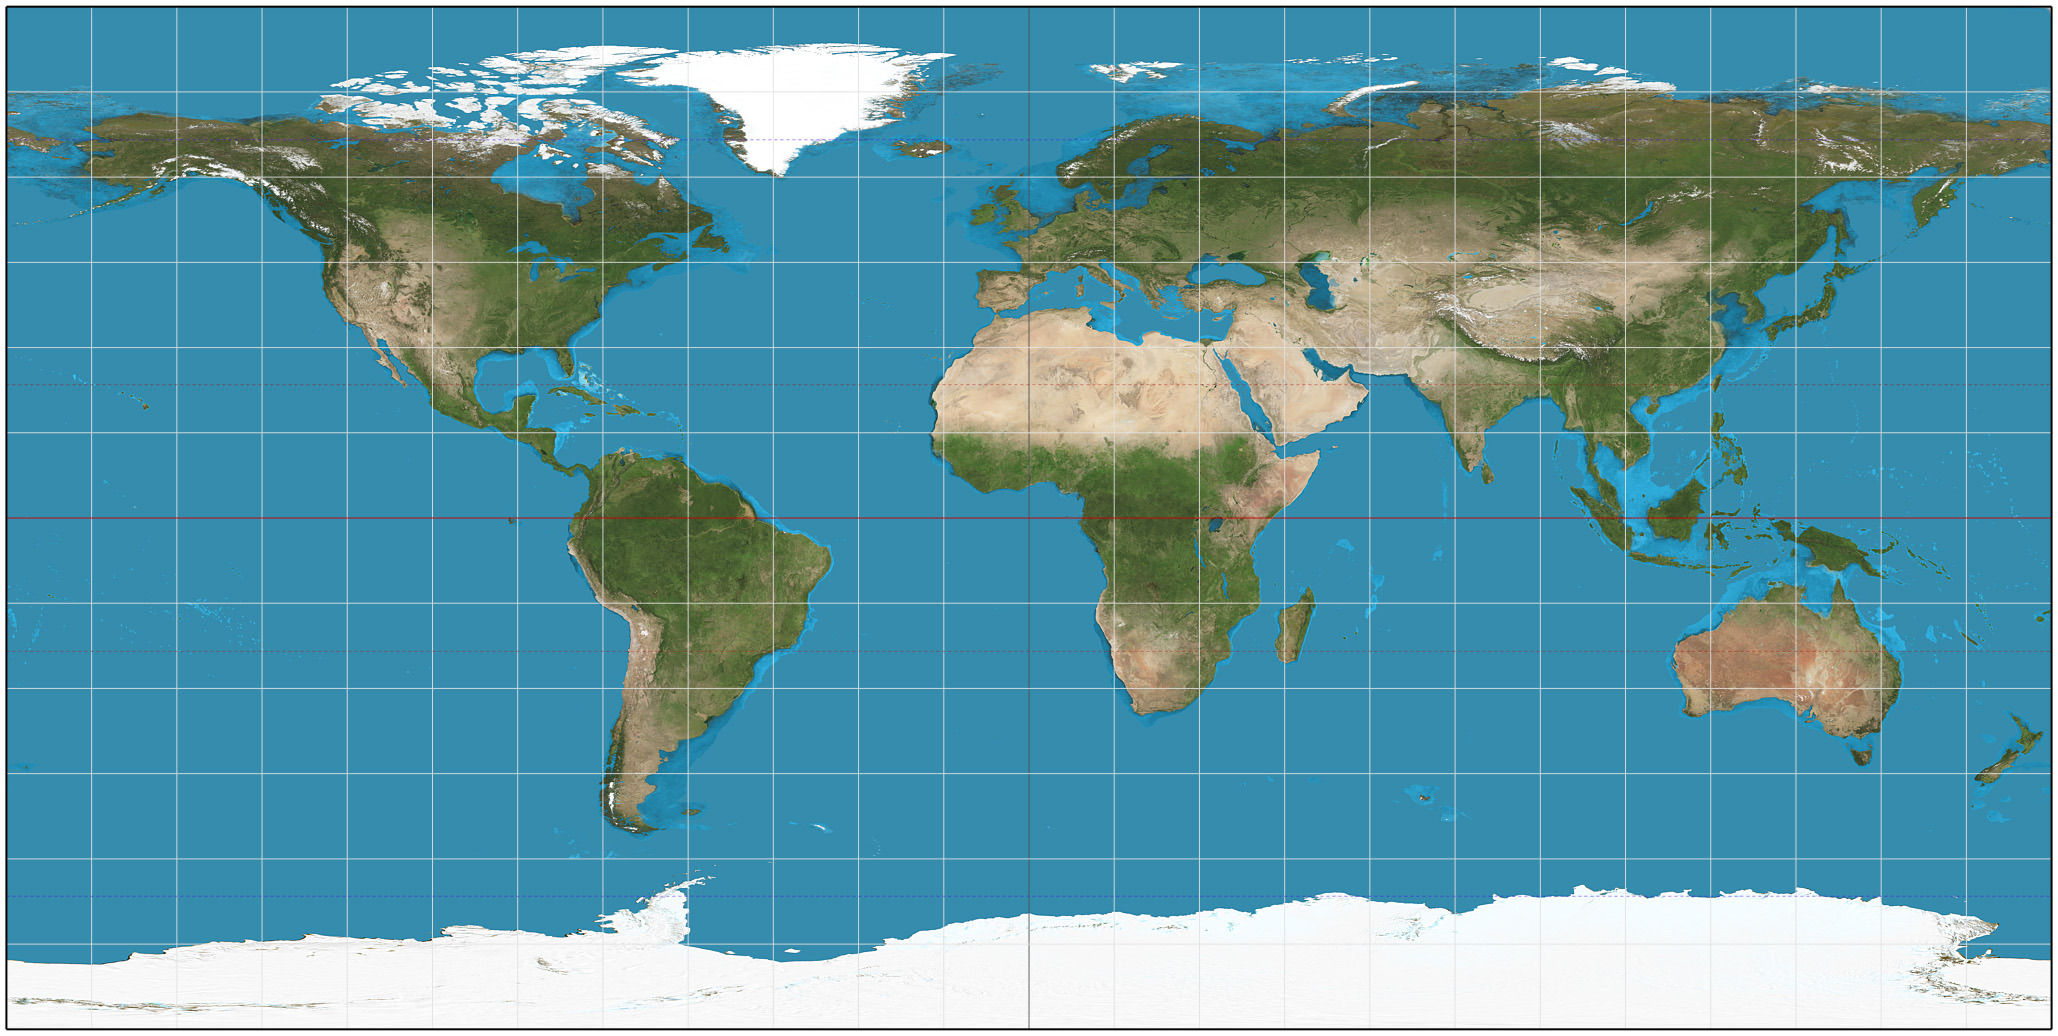
\includegraphics[width=.5\textwidth]{Images/Equirectangular_projection_SW.jpg}
	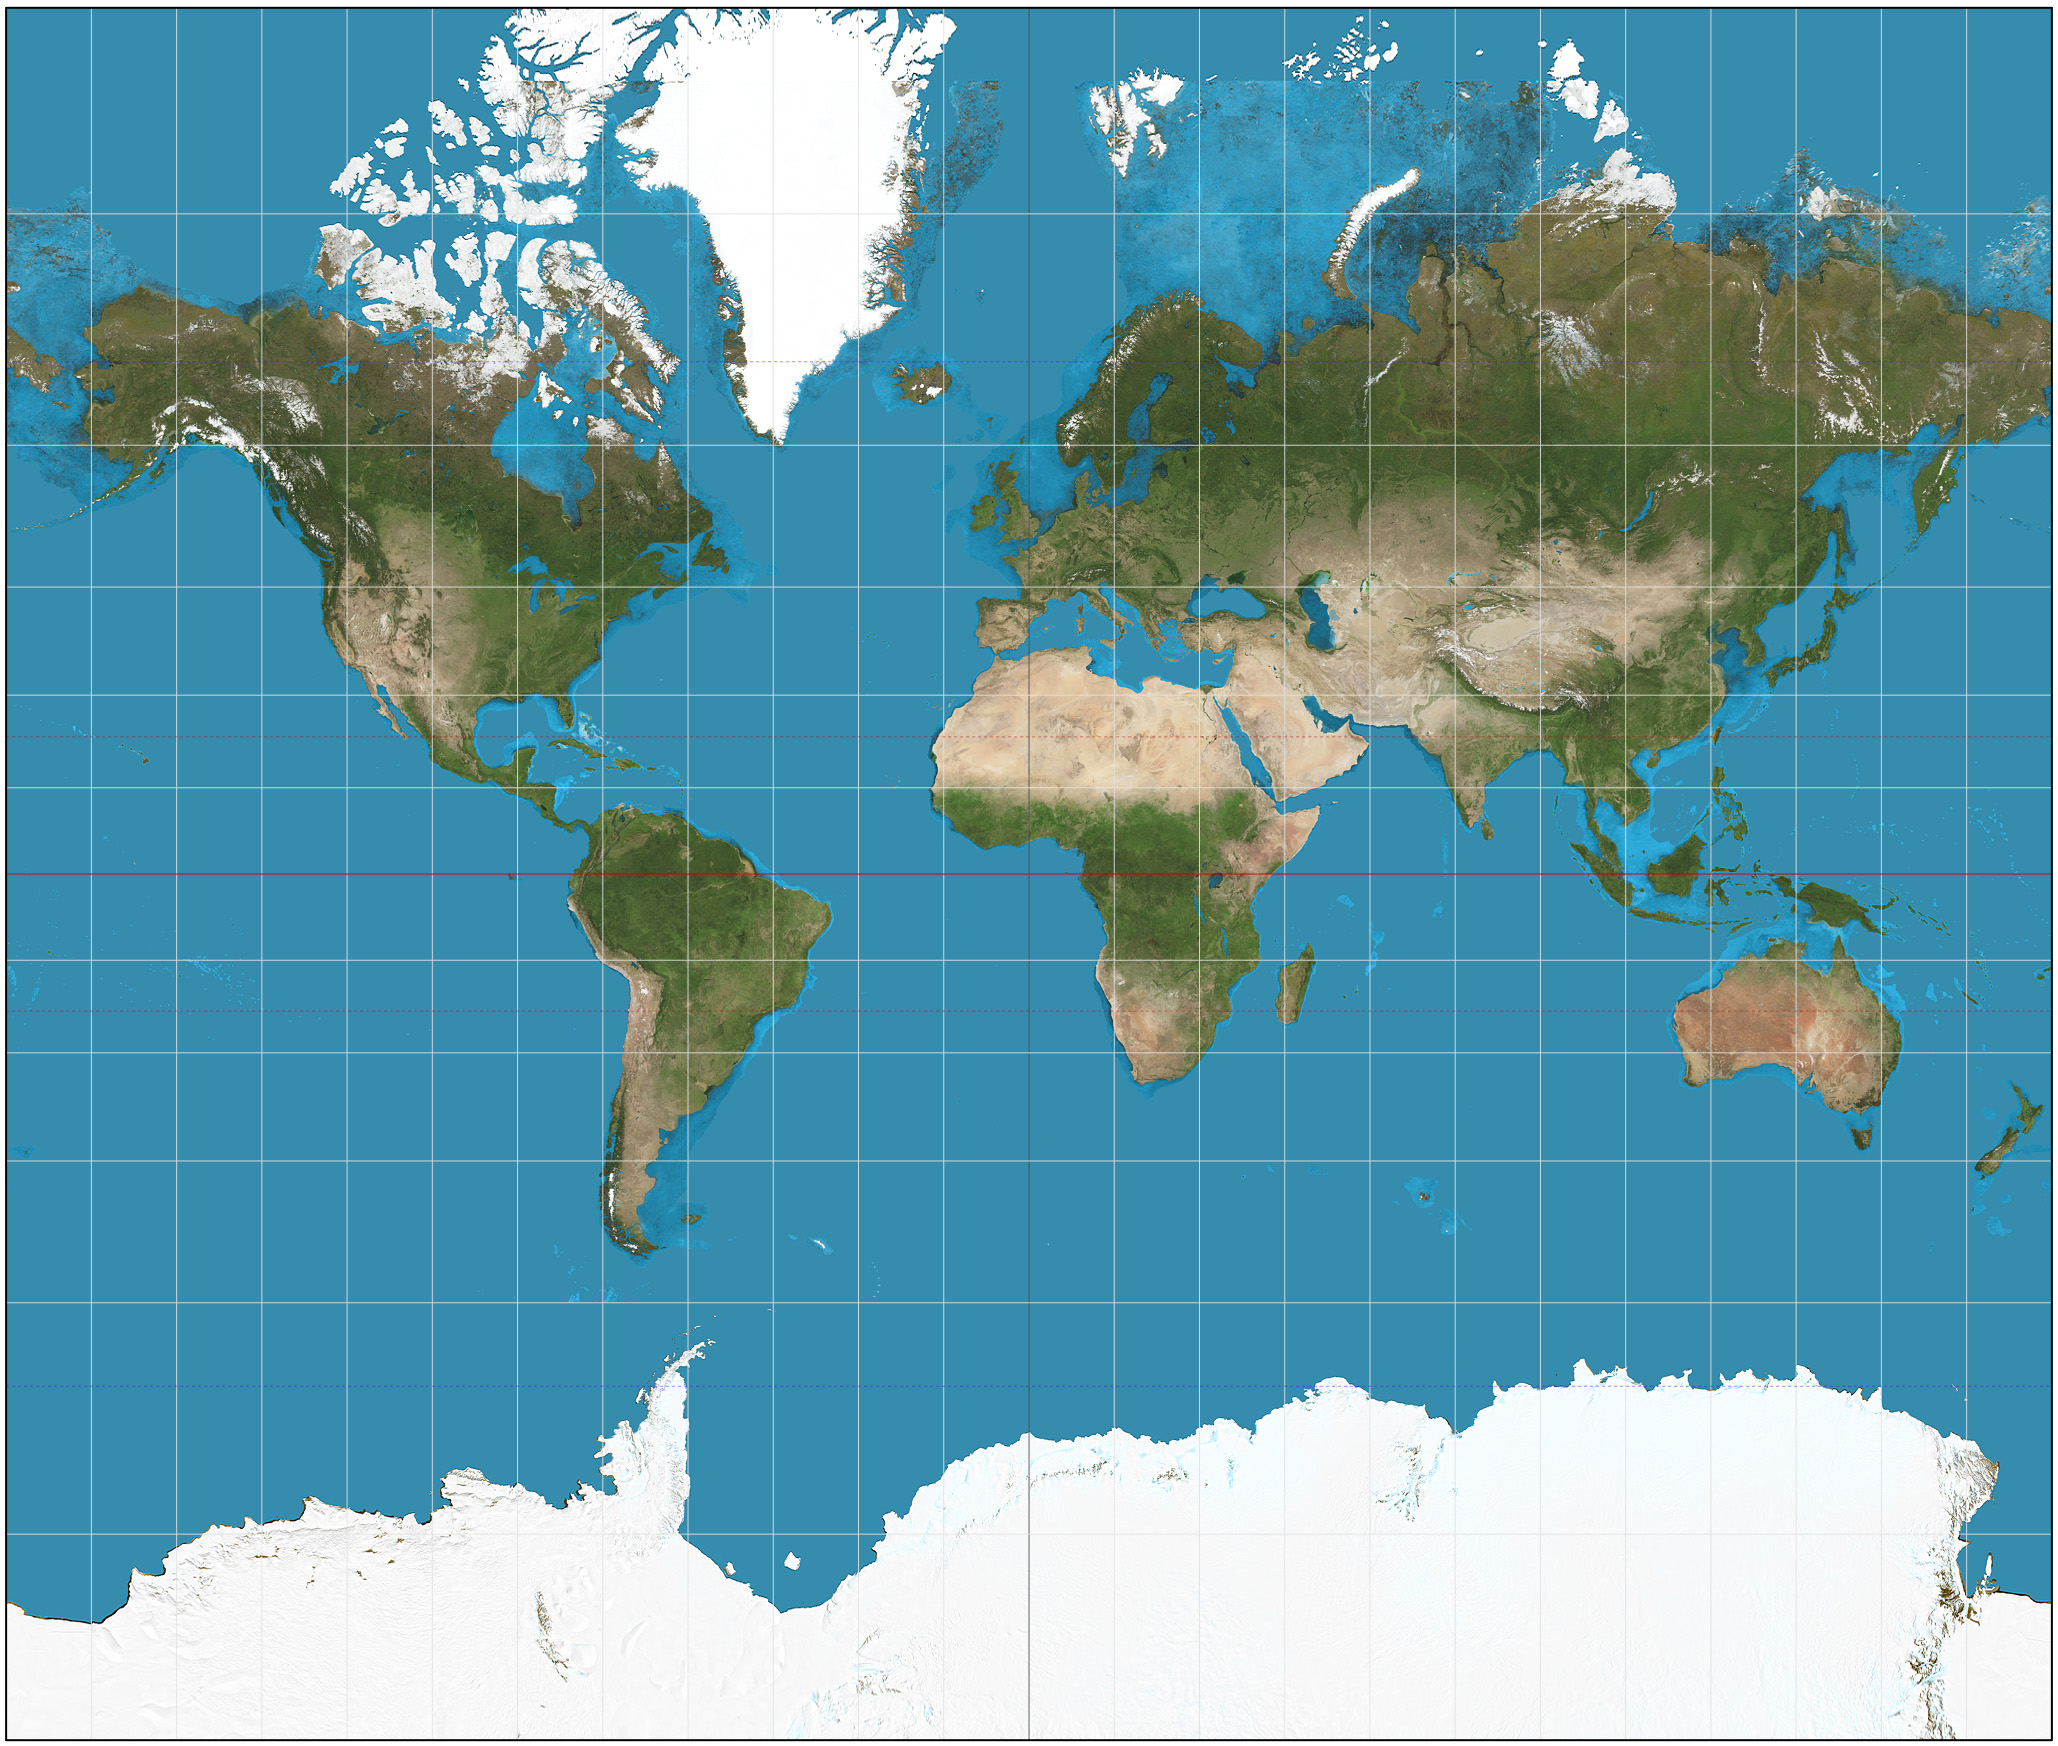
\includegraphics[width=.5\textwidth]{Images/Mercator_projection_SW.jpg}
\caption[]{Equirectangular projection(left) vs. Mercator projection(right)}
\label{fig:projections}
\end{figure}


As we see in \ref{fig:projections} the difference of both projections is not that serious.
The only in extreme northern/southern areas the differencee is clearly visible.
As mercator is used in most notable map representations as for example Google Maps and is often used for navigation it might be desirable to use mercator.
Though most graphs we will be wokring on do not lie in those extreme areas an thus the added value is not worth the added complexity in calculation.
Therefore we will use the Equirectangular projection for our visualization.


\paragraph{Edges}

It is common to display edges as straight lines.
We could try to display the length or even the costs of the edge by bending them depending on the height of the value.
As the air distance between two nodes and the length of the connecting edge does not derrive that much in general we will display edges by simple straight lines in the visualization.


\paragraph{Nodes}

In most visualizations of graph algorithms, that are mainly used for teaching, nodes are represented by circles.
Though those visualizations perform only on small graphs and are went threw step by step.
As we are going to display much bigger graphs we have to take a look at representation of nodes as well.
In our graphs every node is connected to at least one edge. If not, the only way for the node to be accessed during our algorithms would be to be the start or the target node of the algorithm.
As every node belongs to at least one edge a vizual representation of the node itself is redundant, as it is already represented by at least one end of an edge.

\todo{END}


\section{Displaying the Algorithm}

In this section we are going to the core of the visualization. Except of visualizing one state of the graph, we now want to create a way to see graph changes during the algorithm.


\subsection{Basics}

As we want to display a process now, we will move through the algorithm step by step.
For the visualization this would mean for our visualization to start with a white space and then add the processed edges in the order of their appearance during the algorithm.

\begin{figure}[h!]
	\includegraphics[width=.5\textwidth]{Images/placeholder.png}
	\includegraphics[width=.5\textwidth]{Images/placeholder.png}
\caption[]{Two consecutive steps in the visualization}
\label{fig:projections}
\end{figure}

As we see in (Bild oben) stepping threw the algorihtm like this helps to understand how the  search front evolves quite well.
Now we still need to think about which window of the graph we want to show.
Thereby we have to respect that we have to chose the window big enough to see every action happening during the algorithm, but small enough to have as little unused space as possible, when the search front is fully evolved.
\par
Therefore we could on the one hand take the start and the end node as outer points. Then we would try to estimate the most of points of the search front and add a margin depending on this estimation.
\\
On the other hand we can examine all edges processed before we start to visualize the algorithm. Thereby we could find out the exact borders of the search front.

\begin{figure}[h!]
	\includegraphics[width=.5\textwidth]{Images/placeholder.png}
	\includegraphics[width=.5\textwidth]{Images/placeholder.png}
\caption[]{Estimation method with quite a good estimation(left) vs. Preprocessing method(right)}
\label{fig:projections}
\end{figure}

As the second method finds the perfect window to display we definitive would prefer this method over the other though the precision comes with higher costs which will lead to a higher initial loading time of the visualization.
In the following we will continue using the second method as the perfect view is worth the time to us.
\par
Now that we found the snippet we want to display there would still be a possibility to minimize the empty space on our screen.
Currently we are using the same scale on the x-axis and the y-axis. Therefore on one axis there would be empty space.
\todo {Erklärung warum}
Therefore we could also just spread the graph over the whole screen.

\begin{figure}[h!]
	\includegraphics[width=.5\textwidth]{Images/placeholder.png}
	\includegraphics[width=.5\textwidth]{Images/placeholder.png}
\caption[]{Same scaled axes(left) vs. Spreaded axes(right)}
\label{fig:projections}
\end{figure}

As we see in (Image above) this reduces the unused space to a minimum. On the other hand we would loose a lot of unerstandibility, as the length of a line on the screen would indicate the length of the real edge even less.
Therefore we decided to go with the uniformly scaled axes.


\subsection{Displaying the Tiles}

In \ref{specification} we described the importance of the tiles the graph is splitted in. As the tiles are the mayjor cost factor during the algorithm we should definetly respect them in our visualization.


\subsection{Visualizing the Cache}


\section{Compare algorithms}


\section{Miscellaneous}

\chapter{Outlook}
\begin{itemize}
	\item verschiedene Projektionen
	\item knoten anordnen mit kanten mit länge = kosten
	\item different layers
\end{itemize}


% \chapter{The Solutions}
%
% \section{Displaying Edges} \label{edges_only}
% As the nodes and edges seem to be the most important part of an algorithm the first approach of building our visualization was to draw all nodes and edges as soon as they were processed.
%
% \begin{figure}[H]
%     \centering
%     \includegraphics[width = 1.0\textwidth]{placeholder.png}
%     \caption[HPI logo]{\label{fig:edges_only}Edges-only visualization.}
% \end{figure}
%
% As we see the basic search front is shown in this visualization prette good, but every information about the tiles is missing.
% Therefore we start drawing every edge of a blocks as soon as they is accessed the first time.
%
% \begin{figure}[H]
%     \centering
%     \includegraphics[width = 1.0\textwidth]{placeholder.png}
%     \caption[HPI logo]{\label{fig:edges_only_blocks}Modification of the edges-only visualization. Unloaded edges in already loaded blocks are now plottet as gray lines.}
% \end{figure}
%
% As we see it is now possible to see the basic tile strucure the algorithm has to handle but there are still multiple shortcomes.
% When the algorithm watches already explored edges the user doesn't see any movement on the screen.
% Thus a big part of the algorithm stays unvisualized.
% In adition the tile structure is not recognizable on bigger graphs and particular in the inner graph.
%
% \section{Displaying tiles}
% As mentionioned in \ref{edges_only} the tile structure of the map is still not present enough in regard of their role for the algorithm.
% Hence we now want to represent the tiles by rectangles. As base we use the visualization from \ref{edges_only}.
%
% \begin{figure}[H]
%     \centering
%     \includegraphics[width = 1.0\textwidth]{placeholder.png}
%     \caption[HPI logo]{\label{fig:edges_only_blocks} Showing tile borders as soon as the first node was accessed. }
% \end{figure}
%
% By adding the rectangles to the visualization we solved the problem of unrecogniseable tile borders.
% But still there is big part missing in the visaulization-process. The problem of missing movement in the inner graph mentioned in \ref{edges_only} is still present.
% Hence we will take a look at possible solutions in the next sections.
% Since displaying all edges leads to a bad performance on a bigger routes and as they do not really add value to the visualization on a higher level we will continue using only the rectanglerepresentation of the tiles.
%
% \subsection{Time based coloring}
% The first aproach for solving this problem is to
%
% \subsection{Cache based coloring}
%
% \section{Displaying Graph in background}
%
% \section{Diff between Searchfronts}
%
% \section{basic features}
% - zoom\\
% - stepping threw time\\
%



% \chapter{Gedanken}
% NDS motivieren?
% Inwieweit das Projekt erklären?
% Einzelne Features:
% Wie genau auf Algorithmen eingehen?
% Nur verlinken?
% Erst Wünsche an Visualisierung?
%
% Historisch rangehen?\\
%
% Introduction\\
% Graphs important -> developing graph algorithms important -> Bad results/hard to imagine how the algorithm works in reality -> Visualizeing helps to access information -> Visualizing the algorithm -> bachelorproject -> problem -> building a visualization based on problem\\
% Main part\\
% historische rangehensweise? --> Motivation --> resultat --> relektieren --> repeat\\
% Fazit\\
% Resultat verallgemeinern --> Maß zwischen planen und baunen finden --> schnell beginnen --> feedback von nutzern\\
%
% Gliederung
% Einleitung
% Probleme
% 	Graphstruktur
% 	Wie stell ich den Graph dar?
% 		Wo ist welcher Knoten?
%
% 	Wie stelle ich den Algorithmus dar?
% 	Wie beziehe ich die Tiles ein?
% 	Wie stelle ich den Cache dar?
% Lösungen
% Ausblick und Fazit
%
% \chapter{Chapter}
%
% \lettrine[findent = -0.3 em, nindent = 0.7 em]{A}{} small example as proposed by~\citet{test}.\myfootnote[-0.2]{The footnote number shouldn’t be in superscript down here.} Just some text referring to~\Cref{fig:HPI} and citing~\citet{test2}.\myfootnote[-0.2]{And another footnote.}
%
% \begin{figure}
%     \centering
%     
\includegraphics[width = 9 cm]{HPI_Logo.pdf}
%     \caption[HPI logo]{\label{fig:HPI}That’s the logo of the HPI. Naturally, it comes without its obligatory safe zone.}
% \end{figure}
%
% \section{Section}
%
% \subsection{Subsection}
%
% \subsubsection{Subsubsection}
%
% \newpage
% More text.
% \newpage
% Even more text.

% References
\renewcommand*{\bibname}{References}
\bibliographystyle{abbrvnat}
\bibliography{Files/References}


\chapter*{Independence Declaration}
\addcontentsline{toc}{chapter}{Declaration of Authorship}
\thispagestyle{empty}

I hereby declare that the thesis submitted is my own unaided work. All direct or indirect sources used are acknowledged as references.\vspace{2 ex}

Potsdam, \today\\[6 ex]

\begin{flushleft}
    \begin{tabular}{p{5cm}}
        \hline
        \centering\footnotesize\printAuthor
    \end{tabular}
\end{flushleft}


\end{document}
